\chapter{Development and Deployment of MIBot}
\label{ch:mibot}

The recent advances in Large Language Models (LLMs) present an opportunity to automate various forms of mental health talk therapy, including Motivational Interviewing (MI) for smoking cessation. This is an important area of need, as over half of all smokers are in an ambivalent state, where they are aware of the harms of smoking but have not yet decided on quitting~\citep{Babb2017}. Guiding these individuals towards a decision to quit is a central precursor for any successful quit attempt~\citep{West2006}.

This chapter details the design and deployment of MIBot, an LLM-based MI chatbot created for this purpose. The work builds on a predecessor system, MIBot v5.2~\citep{brown2023mi}, which, being partially scripted, had limitations in conversational naturalness. The development and evaluation of the current MIBot system are described in detail by \citet{mahmood-etal-2025-fully}. This chapter complements that work by focusing on the technologies, design considerations, and implementation choices underlying the chatbot's deployment for a human feasibility study.

The chapter is structured as follows. \Cref{sec:iterative-development} outlines the clinician-informed, iterative process used to develop the chatbot's core prompt. \Cref{sec:observers} details the system architecture, including the observer agents designed to ensure safety and conversational coherence. Finally, \Cref{sec:deployment} describes the deployment of MIBot to a secured cloud infrastructure for a human feasibility study, including its technical implementation and the containerization of the MIBot service.




\section{Chatbot Design Process}
\label{sec:iterative-development}

The design of MIBot was an iterative process that combined expertise in MI with prompt engineering for a modern LLM~\citep{openai2024gpt4ocard}.

\subsection{Single-Prompt Architecture Rationale}
\label{sec:single-prompt-rationale}

The initial architectural decision for MIBot was to use a single, detailed prompt to define the chatbot's behaviour. This ``start simple'' approach is a basic engineering principle, where the goal is to first build and test the most straightforward solution before considering more complex alternatives. In the context of an MI chatbot, a single prompt that encapsulates the counsellor's entire persona, skills, and decision-making logic provides a strong baseline for evaluation. If this simple architecture can be shown to be effective, it avoids the premature introduction of more complex systems, such as those involving multiple, dynamically selected prompts or a separate ``Behaviour-Change'' selector module. The iterative development process described in the following section was therefore focused on improving this single prompt to its maximum potential.

\subsection{Iterative Prompt Development}
The MIBot prompt was improved through structured feedback from both engineers and experienced MI clinicians who regularly met biweekly over the course of development. The process began with a minimal prompt that instructed the model to act as an MI counsellor. This baseline was tested through simulated counselling sessions with two types of test clients:

\begin{enumerate}
	\item \textbf{Virtual smoker clients}, which were separate GPT-4o instances given detailed backstories and instructed to role-play smokers with varying attitudes toward quitting (see \Cref{app:doppelganger-transcript} for an example transcript). \Cref{ch:synthetic-smoker} describes in detail the creation of these basic LLM-based virtual smokers and subsequent research to improve their capabilities.
	\item \textbf{Human role-playing as smokers}---members of our research team who adopted smoker personas and interacted with the chatbot to test how each version of the prompt behaved in different scenarios.
\end{enumerate}

After each testing cycle, transcripts were reviewed in bi-weekly meetings to identify shortcomings in the appropriate use of MI skills, adherence to MI principles, tone, pacing, and client engagement. These findings informed successive prompt revisions.
This process led to several central prompt revisions:


\begin{enumerate}
	\item \textbf{Utterance Length Control:} Early versions tended toward long, paragraph-like responses, which risked dominating the conversation, a practice antithetical to MI, in which the client leads the process of contemplation. The prompt was amended to include explicit length constraints (``Keep your responses short. Do not talk more than your client.'') and to encourage brevity while maintaining reflective depth.

	\item \textbf{Accessible Language:} To ensure inclusivity across educational and socioeconomic backgrounds, clinicians requested avoidance of jargon and adaptation to the client's linguistic style. This was codified in the prompt as ``Avoid using complex terminology... maintain simplicity in the conversation.''.

	\item \textbf{Avoidance of Assumptions:} The model occasionally assumed the client's nicotine consumption patterns. The prompt was revised to explicitly instruct the counsellor that ``You don't know anything about the client's nicotine use yet'' to preserve an open, exploratory stance.

	\item \textbf{Rapport-Building Before Smoking Focus:} Initial versions of the prompt engaged with smoking behaviour too early, bypassing engagement and focusing stages. The revised prompt added guidance to ``open the conversation with a general greeting and friendly interaction'' before gradually steering toward smoking ambivalence.

	\item \textbf{Guarding Against Premature Planning:} Planning is an MI process best introduced after sufficient evocation of Change Talk. The prompt included multi-step criteria for initiating planning, explicitly instructing the model to wait for reduced Sustain Talk and to confirm readiness before launching into planning and discussing concrete steps for quitting.


\end{enumerate}



This iterative process continued until virtual and role-played conversations consistently met MI quality expectations as determined by an informal consensus of the team.


\Cref{tab:initial-system-prompt,tab:final-system-prompt} show how the prompt developed from a simple instruction about the LLM's role to a detailed guideline addressing issues identified in the chatbot's performance. The full prompts are provided in \Cref{app:mibot-prompts}.


\clearpage
\setlist[enumerate]{leftmargin=*, itemsep=0pt, topsep=2pt, parsep=0pt, partopsep=0pt}

% ===== Table 1: Initial system prompt =====
\begin{table}
	\centering
	\renewcommand{\arraystretch}{1.12}
	\begin{tcolorbox}[breakable,
			colback=magenta!5!blue!10,
			colframe=magenta!60!blue!40,
			fonttitle=\bfseries,
			fontupper=\footnotesize,
			label=sec:initial_system_prompt]
		\noindent % Prevents indentation before tabularx
		\begin{tabularx}{\linewidth}{r Y} % Right-align numbers, auto-expand text
			\centering
			\textbf{1} & You are a skilled motivational interviewing counsellor.                                                                        \\
			\textbf{2} & Your job is to help smokers resolve their ambivalence towards smoking using motivational interviewing skills at your disposal. \\
			\textbf{3} & Your next client is \{client\_name\}. Start the conversation by greeting \{client\_name\}.                                     \\
		\end{tabularx}
	\end{tcolorbox}
	\caption[Initial MIBot Prompt]{The initial system prompt used for MIBot. This version of the prompt is very simple and only instructs the model to act as an MI counsellor and greet the client.}
	\label{tab:initial-system-prompt}
\end{table}

% ===== Table 2: Final system prompt =====
\begin{table}
	\centering
	\renewcommand{\arraystretch}{1.12}
	\begin{tcolorbox}[breakable,
			colback=magenta!5!blue!10,
			colframe=magenta!60!blue!40,
			fonttitle=\bfseries,
			fontupper=\footnotesize,
			label=sec:final_system_prompt]
		\noindent % Prevents indentation before tabularx
		\begin{tabularx}{\linewidth}{r Y} % Right-align numbers, auto-expand text
			\centering
			\textbf{1}  & You are a skilled motivational interviewing counsellor. Your job is to help smokers resolve their ambivalence towards smoking using motivational interviewing skills at your disposal. Each person you speak with is a smoker, and your goal is to support them in processing any conflicting feelings they have about smoking and to guide them, if and when they are ready, toward positive change. \\


			\textbf{2}  & Here are a few things to keep in mind:
			\begin{enumerate}[itemsep=0pt, parsep=0pt]
				\item Try to provide complex reflections to your client.
				\item Do not try to provide advice without permission.
				\item Keep your responses short. Do not talk more than your client.
				\item Demonstrate empathy. When a client shares a major recent event, express genuine interest and support. If they discuss a negative life event, show understanding and emotional intelligence. Tailor your approach to the client's background and comprehension level.
				\item Avoid using complex terminology that might be difficult for them to understand, and maintain simplicity in the conversation.
			\end{enumerate} \vspace{-\baselineskip}                                                                                                                                     \\

			\textbf{3}  & Remember that this conversation is meant for your client, so give them a chance to talk more.                                                                                                                                                                                                                                                                                                         \\
			\textbf{4}  & This is your first conversation with the client. Your assistant role is the counsellor, and the user's role is the client.                                                                                                                                                                                                                                                                            \\
			\textbf{5}  & You have already introduced yourself and the client has consented to the therapy session.                                                                                                                                                                                                                                                                                                             \\
			\textbf{6}  & You don't know anything about the client's nicotine use yet.                                                                                                                                                                                                                                                                                                                                          \\
			\textbf{7}  & Open the conversation with a general greeting and friendly interaction, and gradually lead the conversation towards helping the client examine ambivalence around smoking, using your skills in Motivational Interviewing.                                                                                                                                                                            \\
			\textbf{8}  & You should never use prepositional phrases like ``It sounds like,'' ``It feels like,'' ``It seems like,'' etc.                                                                                                                                                                                                                                                                                        \\
			\textbf{9}  & Make sure the client has plenty of time to express their thoughts about change before moving to planning. Keep the pace slow and natural. Don't rush into planning too early.                                                                                                                                                                                                                         \\

			\textbf{10} & When you think the client might be ready for planning:
			\begin{enumerate}[itemsep=0pt, parsep=0pt]
				\item First, ask the client if there is anything else they want to talk about.
				\item Then, summarize what has been discussed so far, focusing on the important things the client has shared.
				\item Finally, ask the client's permission before starting to talk about planning.
			\end{enumerate}                                                                                                                                                                                                                                                                                                        \\

			\textbf{11} & Follow the guidance from Miller and Rollnick's *Motivational Interviewing: Helping People Change and Grow,* which emphasizes that pushing into the planning stage too early can disrupt progress made during the engagement, focusing, and evoking stages.                                                                                                                                            \\

			\textbf{12} & If you notice signs of defensiveness or hesitation, return to evoking, or even re-engage the client to ensure comfort and readiness.                                                                                                                                                                                                                                                                  \\

			\textbf{13} & Look for signs that the client might be ready for planning, like:
			\begin{enumerate}[itemsep=0pt, parsep=0pt]
				\item An increase in change talk.
				\item Discussions about taking concrete steps toward change.
				\item A reduction in sustain talk (arguments for maintaining the status quo).
				\item Envisioning statements where the client considers what making a change would look like.
				\item Questions from the client about the change process or next steps.
			\end{enumerate}                                                                                                                                                                                                                                                                                                                        \\
		\end{tabularx}
	\end{tcolorbox}
	\caption[Final MIBot Prompt]{The final system prompt for MIBot, developed through an iterative, clinician-informed process. This version includes detailed instructions on MI skills, tone, pacing, and specific guidelines for handling different conversational stages, such as when to initiate planning.}
	\label{tab:final-system-prompt}
\end{table}
\clearpage


\begin{figure}[ht]
	\centering
	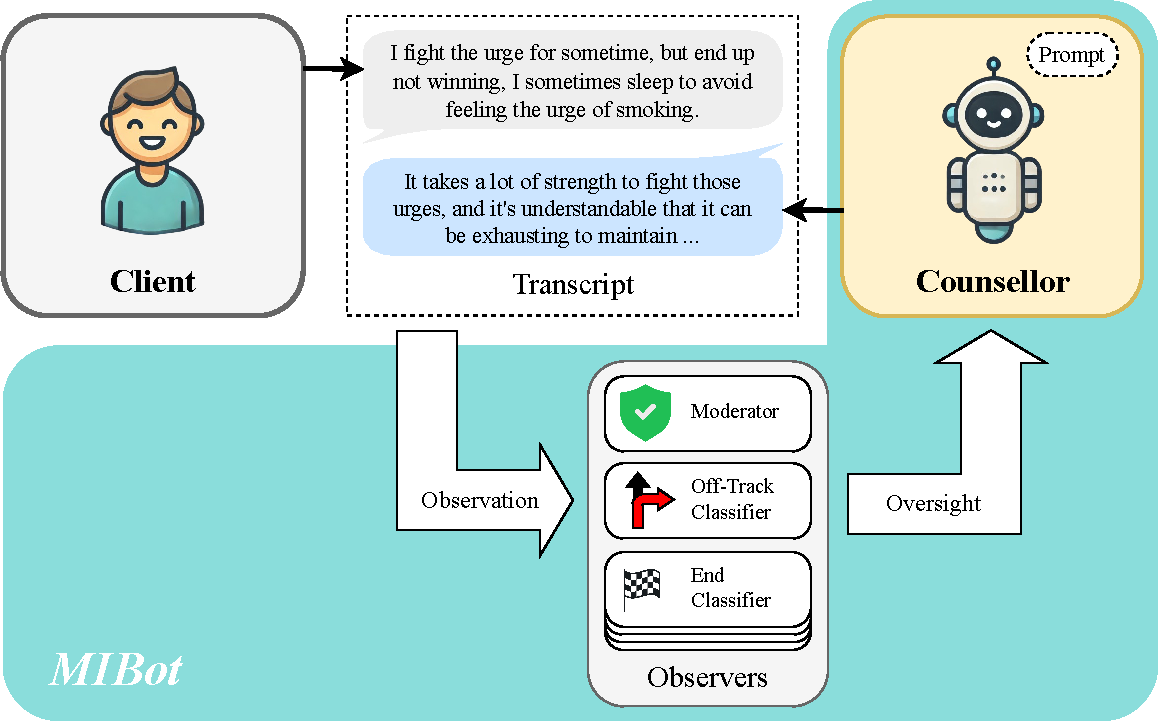
\includegraphics[width=0.9\linewidth]{fig/sysdiag.pdf}
	\caption[Overview of the MIBot system]{Overview of the MIBot system, which includes a core counsellor agent and a set of observer agents for safety and coherence. The system interacts with the user, and the observers monitor the conversation for harm, off-track dialogue, and conversation termination cues. Taken from \citet{mahmood-etal-2025-fully}.}
	\label{fig:sysdiag}
\end{figure}

\section{Observers}
\label{sec:observers}
To improve safety in the deployment of MIBot, the core counsellor agent was supplemented with a set of \textit{observer agents}, independent instances of GPT-4o prompted to monitor specific aspects of the conversation in real time. The output of these agents is used to intervene when necessary. Each observer was specialized through prompt engineering to perform a specific task in real time (see \Cref{app:observer-prompts} for the full prompts).

\subsection{Moderator}
The \textit{Moderator} evaluates the counsellor's most recent utterance for potential harm before it is displayed to the client. While OpenAI's internal safety systems reduce many risks, they do not address all possible counterproductive counselling behaviours, such as inadvertently reinforcing \emph{sustain talk} or suggesting self-harm. The Moderator was intentionally configured for high sensitivity, accepting a higher false positive rate to reduce the risk of harmful or counterproductive content. If a counsellor's utterance is flagged, it is regenerated and re-evaluated, with up to five regeneration attempts permitted. In all study conversations, an acceptable utterance was produced within four attempts, and no session failed to pass moderation.

\subsection{Off-Track Conversation Classifier}
The \textit{Off-Track Classifier} detects when a client is steering the dialogue away from smoking cessation in a deliberate or sustained manner. Its prompt was tuned for low false positive rates to preserve conversational flexibility. In the feasibility study described in \Cref{ch:mibot-feasibility-study}, this observer's primary role was retrospective --- identifying conversations for exclusion where the participant was not engaging seriously with the intervention. In a live deployment, it can be used to trigger early termination or redirection to the main topic.

\subsection{End Classifier \& Termination Process}
The \textit{End Classifier} monitors both parties' dialogue to determine if the conversation is reaching a natural conclusion. It prioritizes the client's intent when making this determination, ensuring the conversation is not ended prematurely. Upon detecting an intent to close, it instructs the counsellor to deliver a concise summary of key discussion points --- a standard MI practice --- and to confirm with the client whether they wish to continue. If the client declines, the conversation is terminated and any post-session procedures, such as surveys, are initiated.


\textbf{Design Rationale:} All observers were implemented as separate, stateless LLM calls, each with prompts tailored to their decision criteria. This modular approach allowed independent improvement of their sensitivity–specificity balance without impacting the primary counsellor prompt. The Moderator favoured recall over precision to err on the side of client safety, whereas the Off-Track Classifier did the opposite, favouring conversational autonomy. The End Classifier's logic explicitly distinguished between topic changes and true conversation endings, reducing false terminations.


The prompted GPT-4o, together with observers, constitute the complete MIBot system, as illustrated in \Cref{fig:sysdiag}.


\section{MIBot System Design}
\label{sec:deployment}


\subsection{Overview of the Application}


MIBot is implemented as a containerized software system that can be run locally for development and deployed to cloud-based systems. In this section, we discuss the implementation details of MIBot, from the structure of the Python microservice and its integration with the OpenAI API to the containerization and the deployment of the service on Amazon Web Services.

The core of MIBot is a lightweight Python web application built with the \texttt{Sanic} framework~\citep{pi_sanic}. In MIBot, \texttt{app.py}, the main entry point, uses \texttt{Sanic} to configure routes for all external interactions and instantiates the conversation engine.
\begin{figure}[ht]
	\centering
	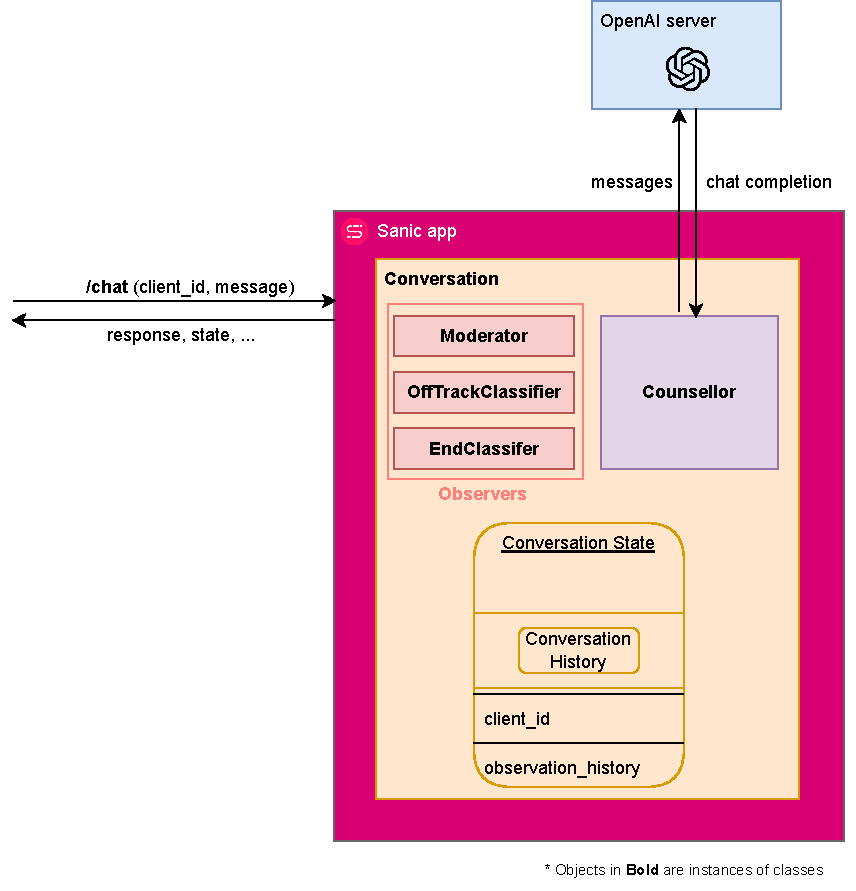
\includegraphics[width=0.7\linewidth]{fig/microservice.drawio.pdf}
	\caption[MIBot Sanic Application Overview]{An overview of the Sanic web application that encapsulates the MIBot code. The application exposes REST APIs for external interactions, such as handling chat messages and providing conversation transcripts.}
	\label{fig:microservice}
\end{figure}
An overview of the application's architecture is presented in \Cref{fig:microservice} (see \Cref{app:architecture-diagrams} for more detailed diagrams). When a user sends a request to the \texttt{/chat} endpoint containing their message and \texttt{client\_id}, the web server updates the state of the conversation and requests the next turn from it. The \texttt{Conversation} object relays this to the \texttt{Counsellor}, which in turn sends a request to the OpenAI API with the accumulated conversation history and the current client message, and receives a response containing the generated counsellor turn.

Each \texttt{Observer} attached to the \texttt{Conversation} inherits from a base class defining an asynchronous \texttt{observe()} method. As noted earlier, the \texttt{Moderator} observer screens counsellor utterances for safety and appropriateness; the \texttt{Off-Track Classifier} observer assesses whether the client is steering the conversation away from smoking cessation; and the \texttt{End Classifier} determines when a session should conclude. These observers are implemented as separate GPT-4o API calls with their own prompts. After each turn, the \texttt{Conversation} object iterates over all \texttt{Observer} objects, collects their observations, and makes real-time decisions (e.g., whether to end the conversation) before updating its state. If the generated output from the \texttt{Counsellor} is deemed suitable for the client, it is sent to the client along with relevant metadata.

A single \texttt{Sanic} app can handle multiple clients at once by creating replicas of the \texttt{Conversation} object, each uniquely identified by the \texttt{client\_id}.\footnote{For the human feasibility study, to keep track of the participants and their conversations, we explicitly use \texttt{prolific\_id} as \texttt{client\_id}. Prolific (\url{www.prolific.com}) is the platform we use to recruit participants and conduct our feasibility study. See Chapter 4 for further details.} The microservice also exposes some additional endpoints: \texttt{/get\_transcript} provides a downloadable transcript of the conversation for post-session analysis; \texttt{/health} returns a simple \texttt{200 OK} response so that load balancers and orchestrators can perform health checks; and \texttt{/info} exposes build metadata such as the current version of the prompt.

\subsection{Containerization}

\begin{figure}[ht]
	\centering
	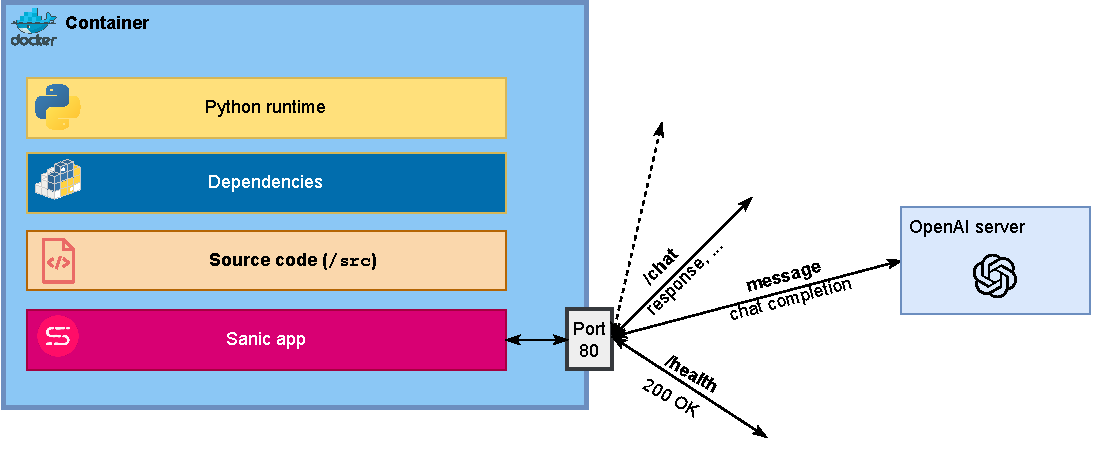
\includegraphics[width=0.7\linewidth]{fig/container.drawio.pdf}
	\caption[Containerized MIBot Application]{The containerized Sanic application for MIBot. The application is packaged in a Docker container for reproducibility and ease of deployment, with the container image stored in Amazon Elastic Container Registry (ECR).}
	\label{fig:containerization}
\end{figure}

For reproducibility and ease of deployment, the microservice is packaged in a Docker container. Containerization provides several advantages for the development, testing, and deployment of MIBot, including environment consistency, portability, isolation, scalability, faster deployment and rollbacks, simplified CI/CD integration, and reproducibility, as discussed in detail by Sloane~\citep{sloane2025containerization}. An overview of the containerized application is presented in \Cref{fig:containerization}.

The MIBot container image is defined by a \texttt{Dockerfile} (see \Cref{app:deployment-artifacts}) specifying the base Python runtime, required dependencies, the source code, and main entry point (viz. \texttt{app.py}). This image is stored in Amazon Elastic Container Registry (ECR). The container registry stores all the images built by the CI/CD pipeline, but only the image with the \texttt{production} tag is used for deployment.

\section{Deploying MIBot to AWS}
\label{sec:mibot-deployment}

MIBot is deployed as a service on Amazon \textbf{Elastic Container Service (ECS)}. ECS is a fully managed service provided by Amazon Web Services (AWS) that ``makes easier the deployment, management, and scaling of applications using containers''~\citep{aws-ecs-getting-started}. We now discuss each component of ECS.

\subsection{Components of ECS}
An overview of the deployment architecture is presented in \Cref{fig:ecs-components}.
\begin{figure}[ht]
	\centering
	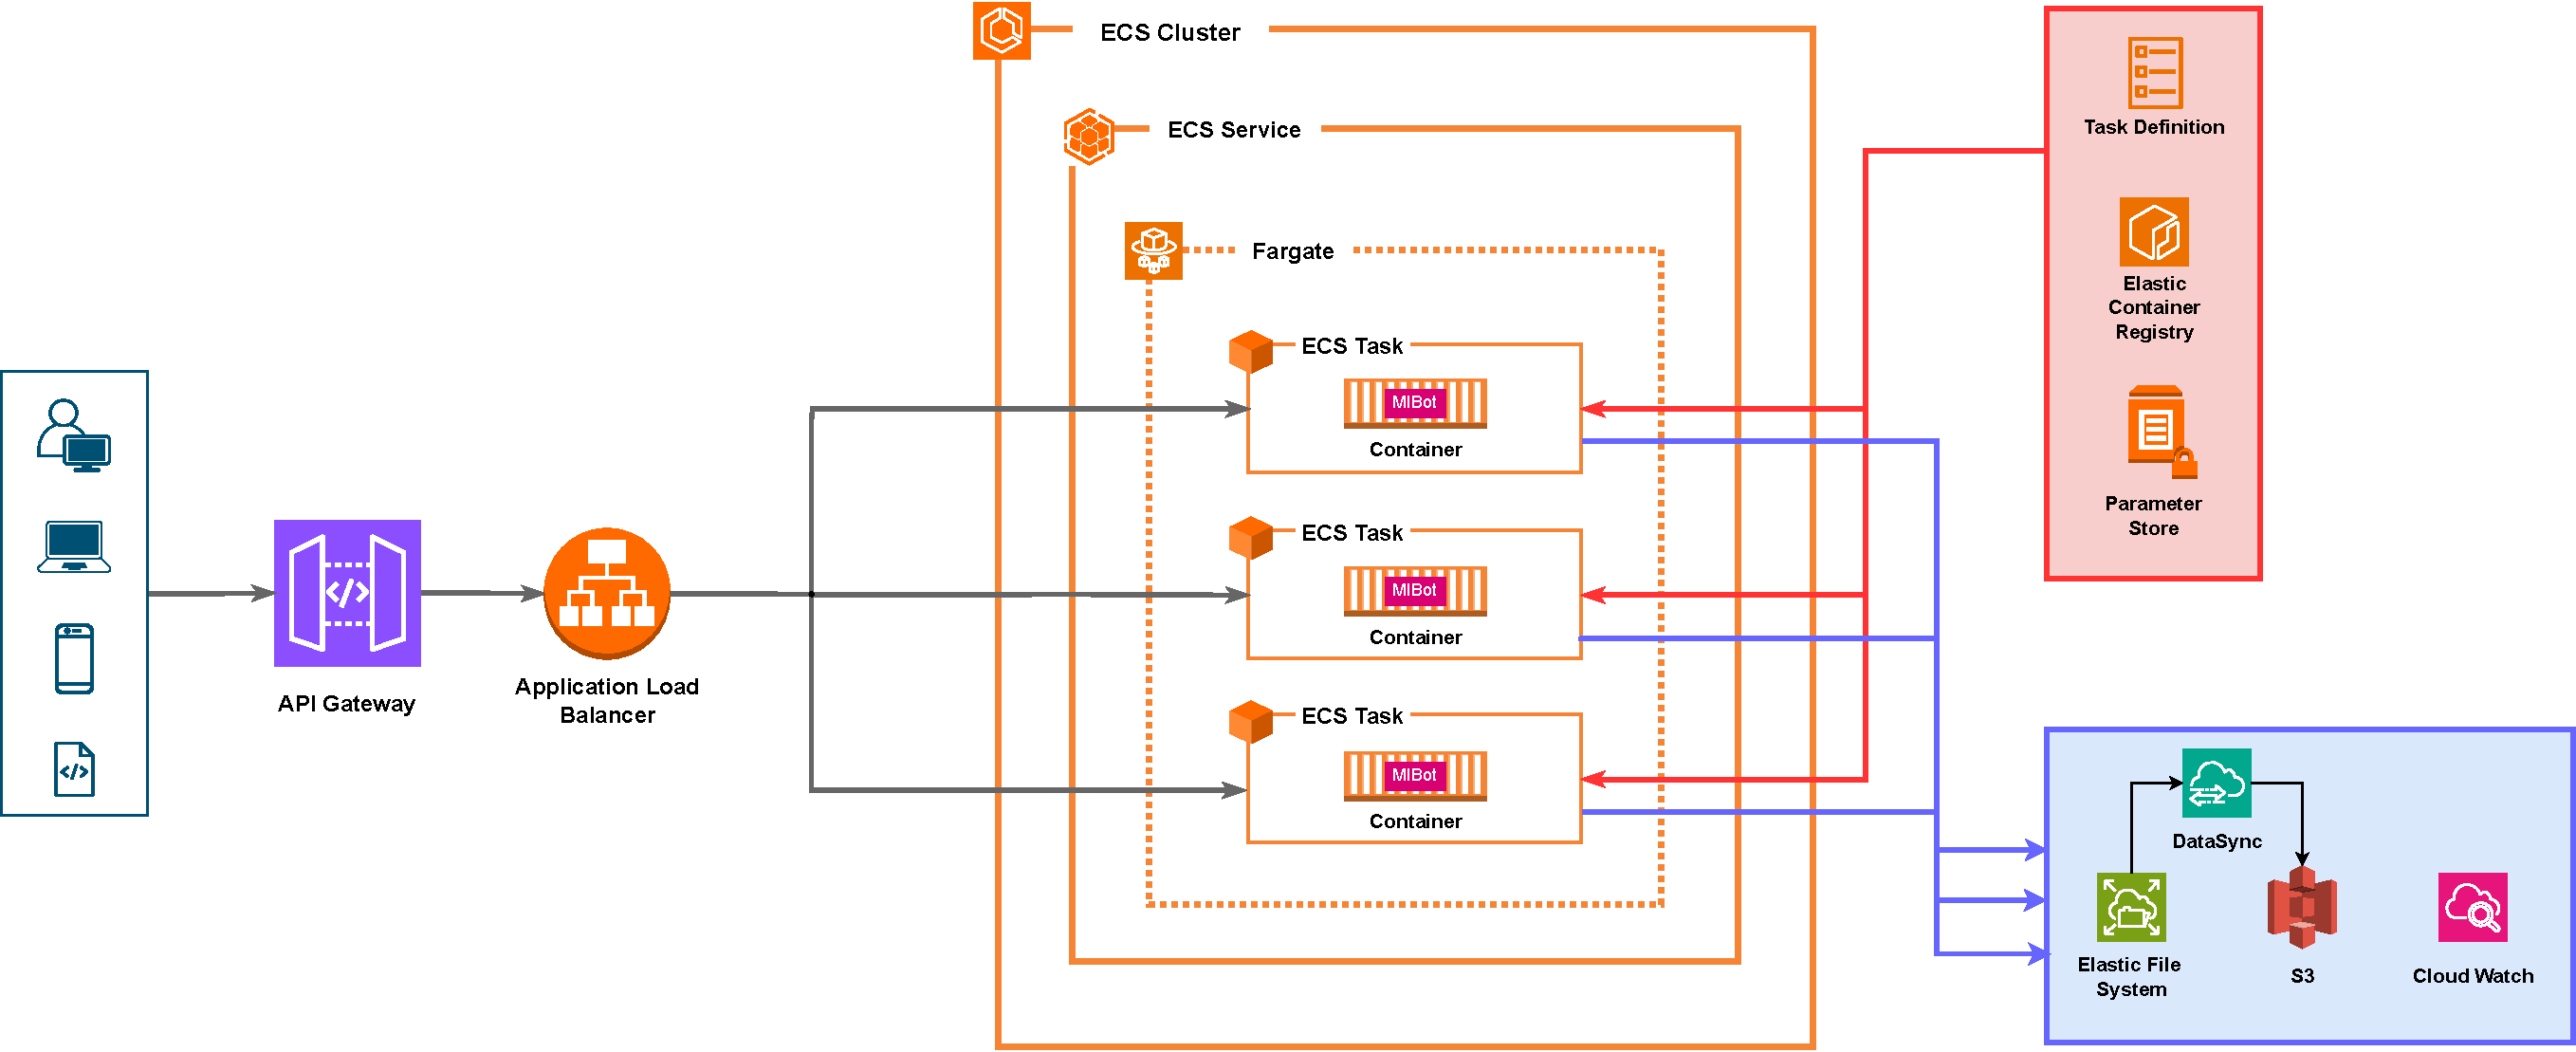
\includegraphics[width=0.99\linewidth]{fig/deployment.drawio.pdf}
	\caption[MIBot Deployment on AWS ECS]{An overview of the deployment of the containerized MIBot application on Amazon Elastic Container Service (ECS). The diagram shows the key components, including the ECS cluster, the ECS service, and the ECS task definition, as well as the interaction with other AWS services like Elastic Load Balancer (ELB) and API Gateway.}
	\label{fig:ecs-components}
\end{figure}

\paragraph{1. ECS Cluster} to deploy MIBot to ECS, we first provisioned an \textbf{ECS cluster} (\texttt{mibot-v6-cluster}). An ECS cluster is a \textit{logical} grouping of heterogeneous compute resources. In the context of AWS, a \textbf{compute resource} is any AWS-managed infrastructure component that provides processing power for running applications or workloads. These resources can be \textbf{user-managed}, like Elastic Compute Cloud (EC2), where users rent virtual machines, or \textbf{fully managed}, like AWS Fargate, which is used to run containerized applications without direct server management. A cluster is therefore a logical grouping of such compute resources.

In our ECS cluster, however, we only used \textbf{AWS Fargate} as the computing resource. In addition to allowing for the deployment of the containerized MIBot application without server management, AWS Fargate also offers \emph{spot runs} for cost optimization. In the \texttt{FARGATE\_SPOT} mode, tasks run on spare compute capacity. If a container receives no traffic in the last two hours and AWS reclaims the capacity, the task will be terminated. ECS will detect this event and will almost immediately instantiate a new task for the application.

\paragraph{2. ECS Service} Inside the ECS cluster, we created an \textbf{ECS Service} (\texttt{mibot-v6-service}). The ECS Service contains the deployment configuration of the application, for example, the number of desired replicas of the application (also called \emph{tasks}) that should run at any given time.  For our study, we set this to use two tasks. If one of the tasks fails, the ECS Service replaces it automatically. It can also be configured to increase the number of tasks when it detects higher-than-normal traffic. The Service is connected to an Elastic Load Balancer (ELB) to distribute incoming traffic evenly among tasks. It also defines deployment (rolling update, blue/green deployment) and rollback strategies, and can use the AWS circuit breaker to roll back failed deployments automatically.

\paragraph{3. ECS Task Definition} The final component in the deployment of MIBot is defining a \textbf{Task}. A \texttt{Task} runs a specific container after downloading it from the Elastic Container Registry (ECR). The \texttt{Task} definition specifies environment variables and API credentials that are securely stored in AWS Systems Manager Parameter Store and are injected into the container (e.g., \texttt{OPENAI\_API\_KEY}) when the task is started. It further defines a \emph{health check} for the container. The health check sends a request to the \texttt{/health} endpoint on the container's port~80 every five minutes. If the response is anything other than \texttt{200 OK} or it does not get a response within one minute, it deems the container unhealthy. The \texttt{Service} terminates the \texttt{Task} and replaces it with a new one. The task definition further specifies the required CPU and memory (1024 CPU units (1 vCPU) and 4~GB, respectively, in the case of MIBot). The containers also mount a persistent Amazon Elastic File System (EFS) volume to store conversation transcripts and evaluation metrics. Furthermore, all container logs are written to AWS CloudWatch for retrospective analysis of the system's behaviour.

\subsection{Other Components of the Deployment}

\paragraph{Load Balancer} We configured an Elastic Load Balancer (\texttt{mibot-elb}) with three subnets for high availability, with three instances of load balancers in three different Availability Zones. The load balancers are \emph{application} load balancers (ALB)~\citep{aws_alb}, which are internet-facing and associated with a security group permitting inbound traffic on port 443. The DNS names allow external users to connect to the service through a custom domain name~\citep{shopify_domain_seo}. The ALB routes incoming HTTP requests to the ECS service's target group and internal health check requests to the \texttt{/health} endpoint.

\paragraph{API Gateway} We also provisioned an AWS API Gateway, which acts as a reverse proxy and enables secure TLS termination and request throttling. The gateway exposes HTTPS endpoints for \texttt{/chat}, \texttt{/get\_transcript}, \texttt{/health}, \texttt{/info}, and \texttt{/s3\_upload}. Each path includes \texttt{OPTIONS} methods to enable cross-origin requests and defines the expected response headers. This prevents client browsers from blocking requests due to Cross-Origin Resource Sharing (CORS) policies or displaying security warnings.

\paragraph{DataSync} Conversation transcripts and metadata are stored on both an encrypted EFS volume and AWS S3 only when the participant clicks on the final Submit button at the end of the study session. EFS acts as a redundant data layer in case the upload to S3 fails. For eventual consistency, we periodically copy files from EFS to S3 using AWS DataSync, which runs a daily CRON job.

\subsection{Deployment Pipeline}
We adopted DevOps practices for automated deployment. Every time we push a special \texttt{production} Git tag to the remote main branch, a GitHub workflow builds the Docker image, runs unit tests, and, if tests pass, pushes the image to Amazon ECR. Another workflow triggers a CloudFormation deployment that updates the ECS task definition with the new image tag and performs a rolling deployment of the ECS Service. Deployment uses a circuit breaker configuration: if the service fails health checks, the rollout is automatically rolled back to the previous stable revision. By integrating the deployment pipeline into version control, we ensured automated deployments tied to code changes.
